%*******************************************************************************
%*********************************** First Chapter *****************************
%*******************************************************************************

\chapter{Introduction}  %Title of the First Chapter

\graphicspath{{Chapter1/Figs/}}


%********************************** %First Section  **************************************

\section{Motivation}

Vision is the process of discovering from images what is present in the world and where it is \citep{marr1982vision}. It is an extremely complicated sense, but provides the most powerful cues of our environment. Our eyes capture ten gigabits per second of information from the world around us \citep{anderson2005directed}. The human brain is able to process over three million bits per second of this information \citep{anderson2005directed}. Our brain can use this information to learn a remarkably rich representation of the world around us \citep{barlow1989unsupervised}. However, developing an artificial system which can achieve the same performance and robustness as humans has long challenged researchers from fields as diverse as physiology, philosophy, psychology, engineering, computer science and artificial intelligence.

Computer vision is a multidisciplinary science that strives to give machines the ability to see \citep{szeliski2010computer}. 
This problem is particularly challenging because of the vast complexity and variation in appearance we observe from our visual world. 
To date, designing a hand-engineered approach has not been able to scale to a satisfactory level of understanding \citep{roberts1963machine,papert1966summer}. 
Machine learning techniques \citep{bishop2006pattern} provide the most promising approach for designing systems with human-level understanding of imagery.

As a science, computer vision is having a profound impact on many disruptive areas of technology. The contributions of this thesis are novel machine learning architectures which address many of the core computer vision problems. The architectures proposed in this work are practical, real-time systems which are influencing the development of today’s technology, including autonomous vehicles, augmented reality, medical imaging, drones and smart-city infrastructure. Moreover, being able to build intelligent vision models may contribute to our understanding of the neuroscience behind visual intelligence \citep{sterling2015principles}.

\section{Approach}

\textit{Deep learning} \citep{goodfellow2016deep} is now ubiquitous in the field of computer vision. As a machine learning tool, deep neural networks are very effective at understanding high-dimensional data, such as images. They learn representations by encoding the input through a number of non-linear layers and sub-sampling operations, resulting in powerful image-level understanding and recognition capabilities.
Deep learning models were first used in computer vision for image recognition tasks \citep{lecun88,krizhevsky2012imagenet}.
However, the science of computer vision aims to build machines which can see. This requires models which can extract richer information from images and video than recognition. In general, applying these deep learning models from recognition to other problems in computer vision is significantly more challenging.

This thesis shows how to formulate deep learning models for many core computer vision tasks, and advances the state-of-the-art of each task with practical, real-time models:
\begin{enumerate}
\item Semantic segmentation (what is around us),
\item Instance segmentation (where objects are),
\item Monocular metric depth (how far away objects are),
\item Camera pose (where we are),
\item Stereo disparity (depth from binocular vision),
\item Optical flow (motion of objects in an image),
\item Video semantic segmentation (where objects are in video).
\end{enumerate}
An overview of these results is given in \cref{ch1:teaser}. Collectively, these new methods advance state-of-the-art, with many out-performing previously published approaches to these problems.

The algorithms we propose rely on deep learning \citep{hinton2006fast}. Deep learning has emerged as a powerful paradigm for understanding high dimensional data, such as visual imagery. It is now the core technology behind natural language understanding \citep{sutskever2014sequence}, image recognition \citep{krizhevsky2012imagenet}, speech recognition \citep{hinton2012deep} and many other challenging, high dimensional problems in biology and physics \citep{leung2014deep,helmstaedter2013connectomic,ciodaro2012online}.

Deep learning models form hierarchical layers of increasing levels of abstraction \citep{goodfellow2016deep}. These models are typically optimised by propagating a training signal from the output all the way to the input. This is known as end-to-end learning. 
End-to-end learning models have many advantages. Firstly, they can obtain higher performance by optimising all layers with regards to the end goal. Secondly, they are more scalable and can reduce engineering effort by enabling learning from vast amounts of training data. We show that we can formulate and train models on many computer vision tasks with end-to-end learning, outperforming prior approaches.

\begin{figure}[t]
\centering
    \begin{subfigure}[b]{0.65\textwidth}
\centering
        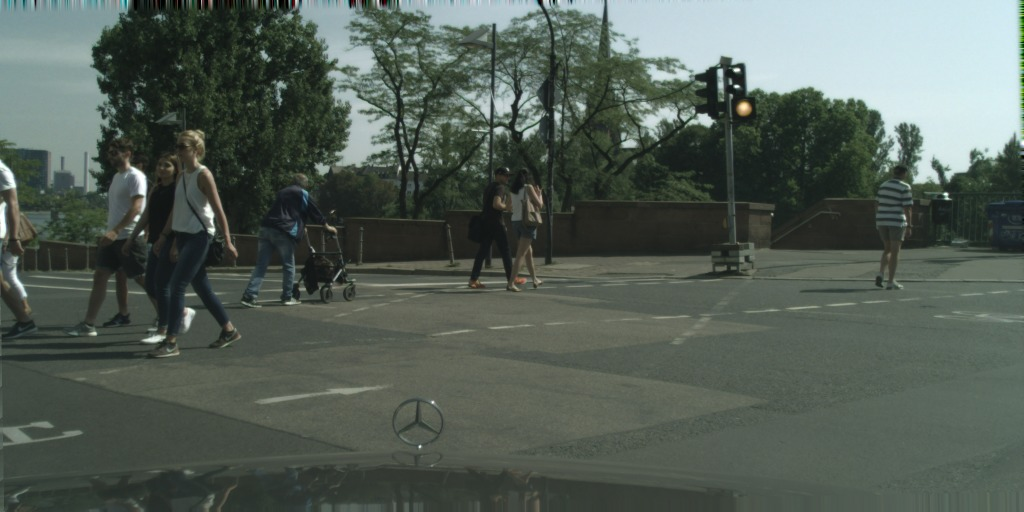
\includegraphics[width=0.48\textwidth,trim={0 20mm 0 0},clip]{segnet_114_output_0.jpg}
        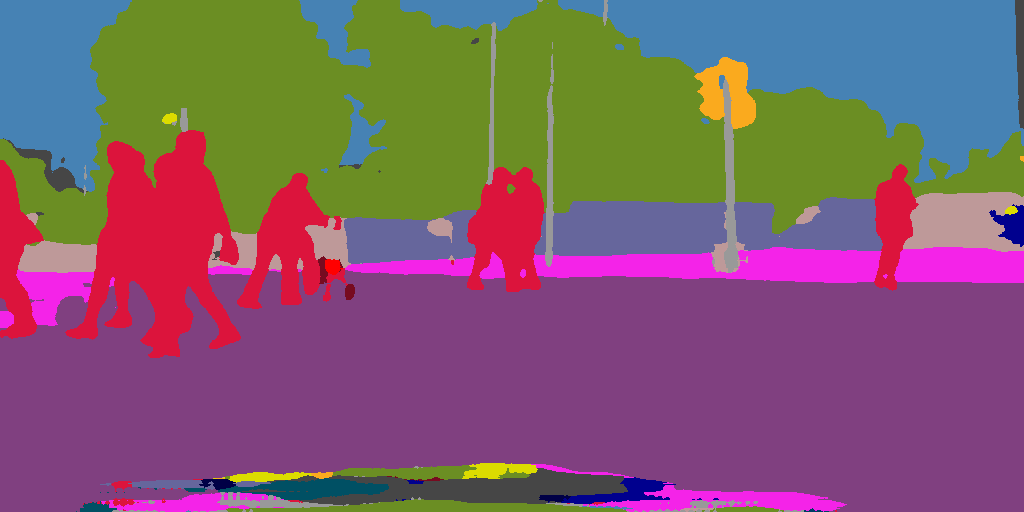
\includegraphics[width=0.48\textwidth,trim={0 20mm 0 0},clip]{segnet_114_output_1.png} \\
        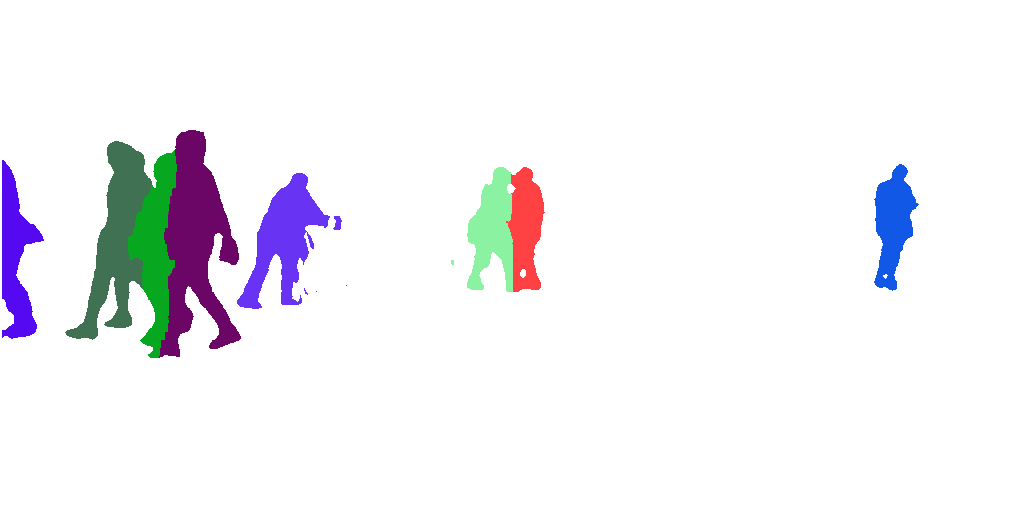
\includegraphics[width=0.48\textwidth,trim={0 20mm 0 0},clip]{segnet_114_output_3.png}
        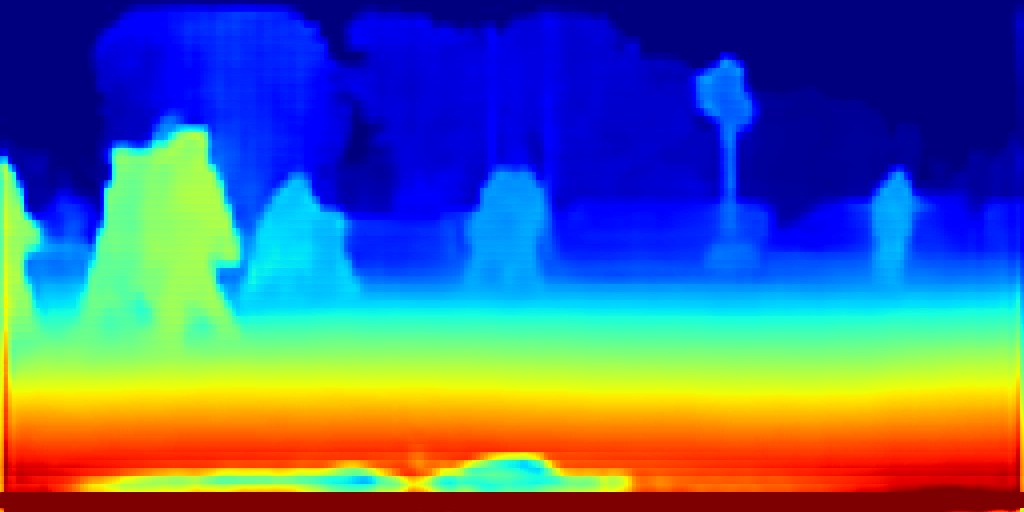
\includegraphics[width=0.48\textwidth,trim={0 20mm 0 0},clip]{segnet_114_output_4.png}
        \caption{Scene Understanding --- understanding the geometry and semantics of a scene. Clockwise from top-left: input image, semantic segmentation, depth prediction, instance segmentation.}
    \end{subfigure}
    \quad
    \begin{subfigure}[b]{0.3\textwidth}
\centering
        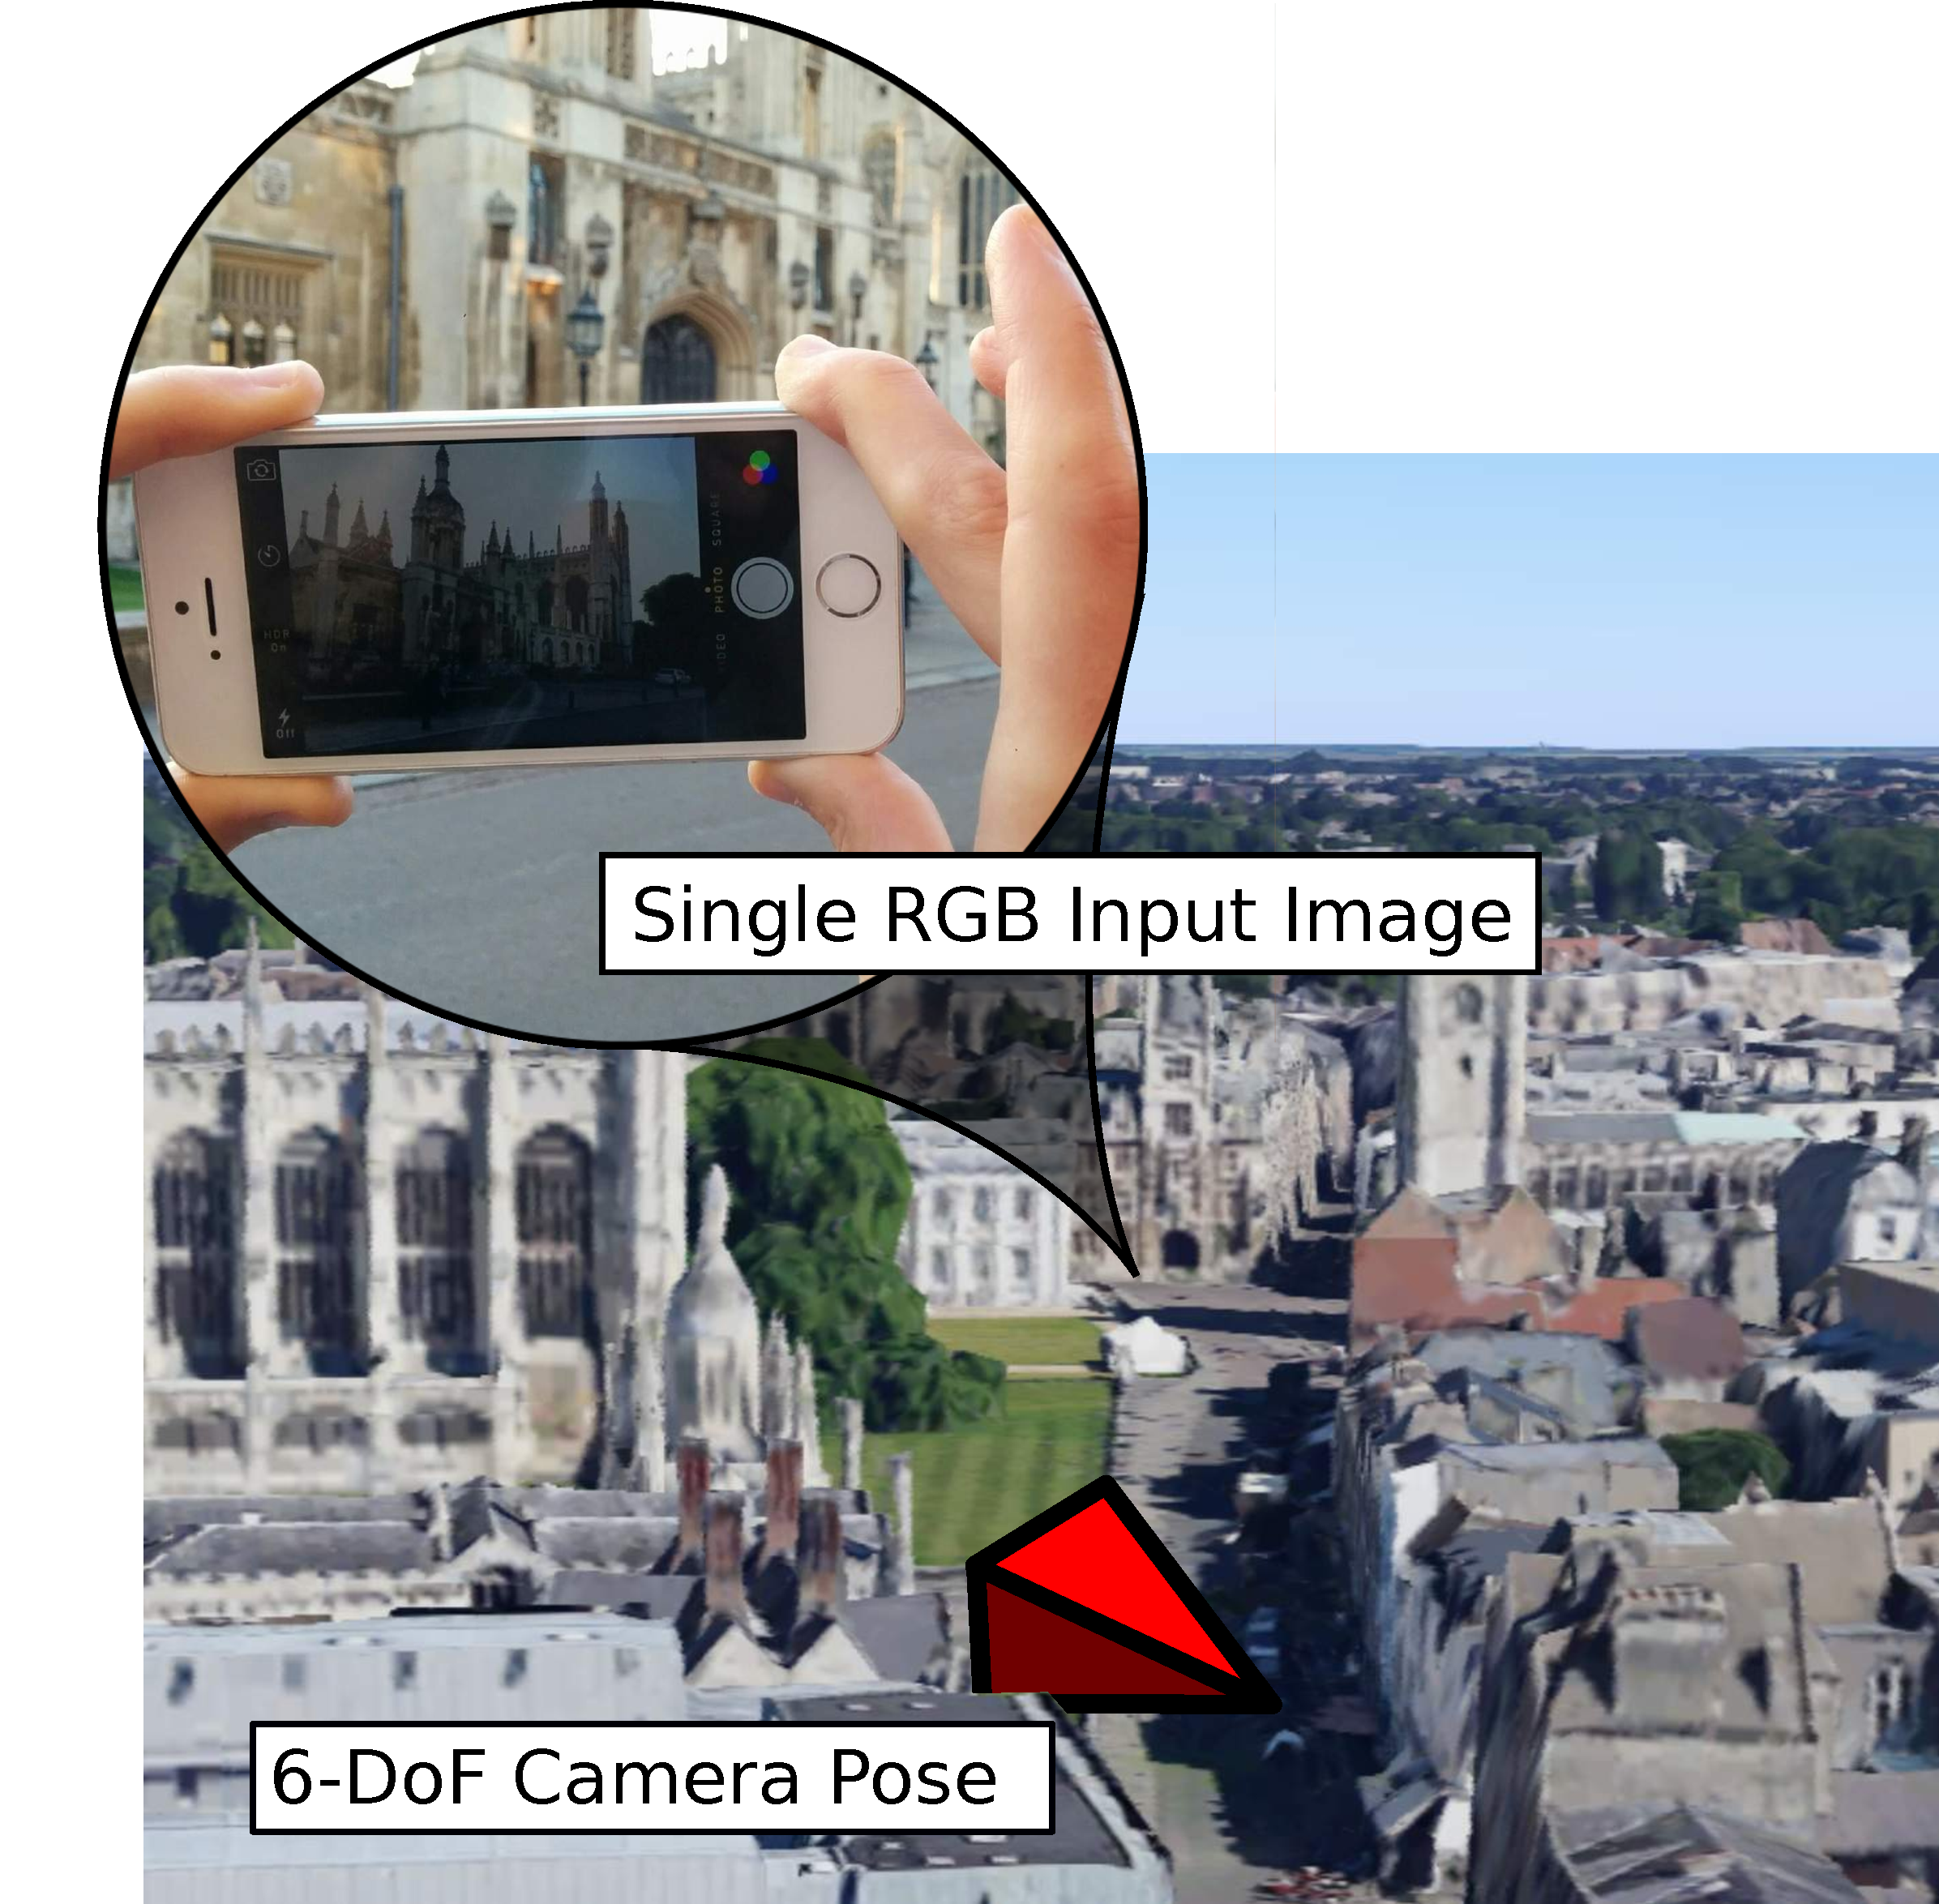
\includegraphics[width=\textwidth]{teaser.pdf}
        \caption{Localisation --- estimating the camera's 3D position and orientation from an image.}
    \end{subfigure}
    
    
    \begin{subfigure}[b]{\textwidth}
\centering
        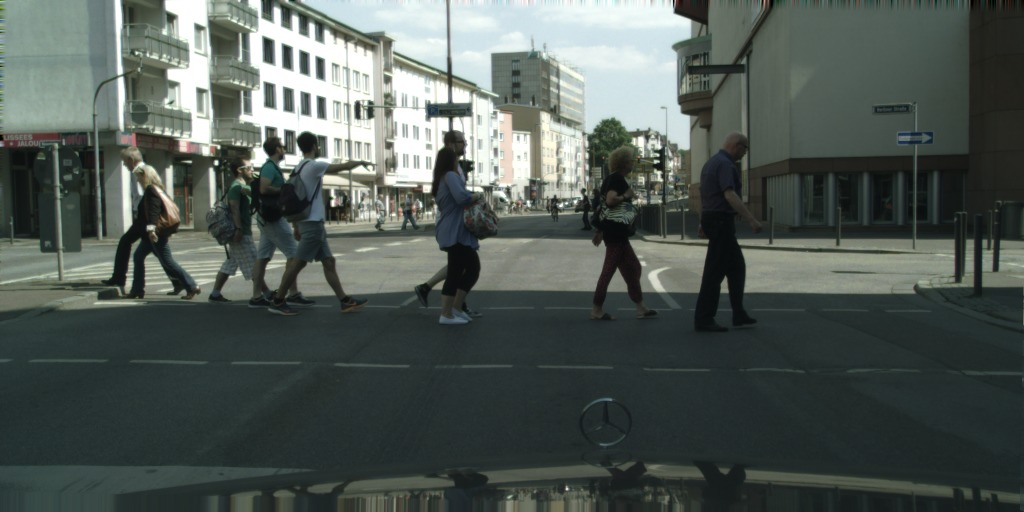
\includegraphics[width=0.32\textwidth,trim={0 20mm 0 0},clip]{Chapter2/Figs/results/segnet_107_output_0.jpg}
        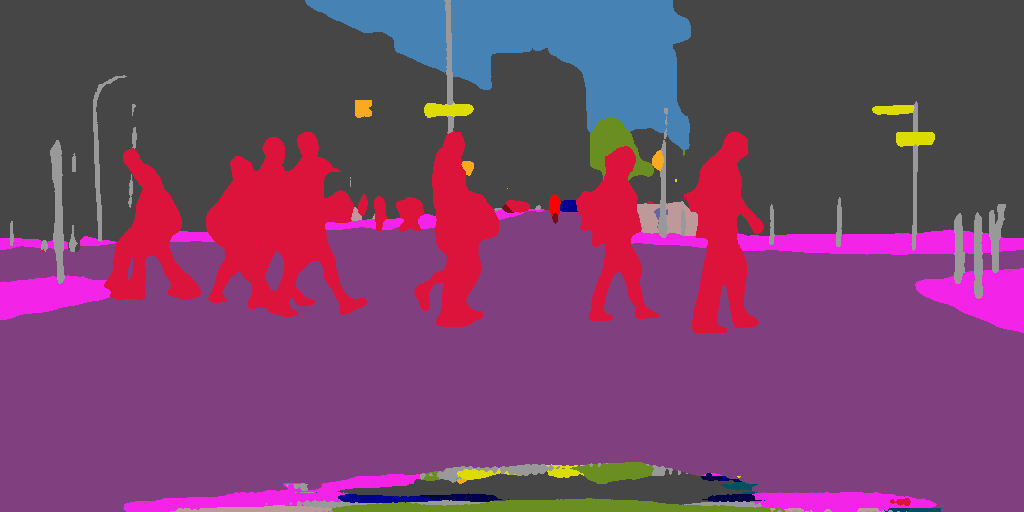
\includegraphics[width=0.32\textwidth,trim={0 20mm 0 0},clip]{Chapter2/Figs/results/segnet_107_output_1.png}
        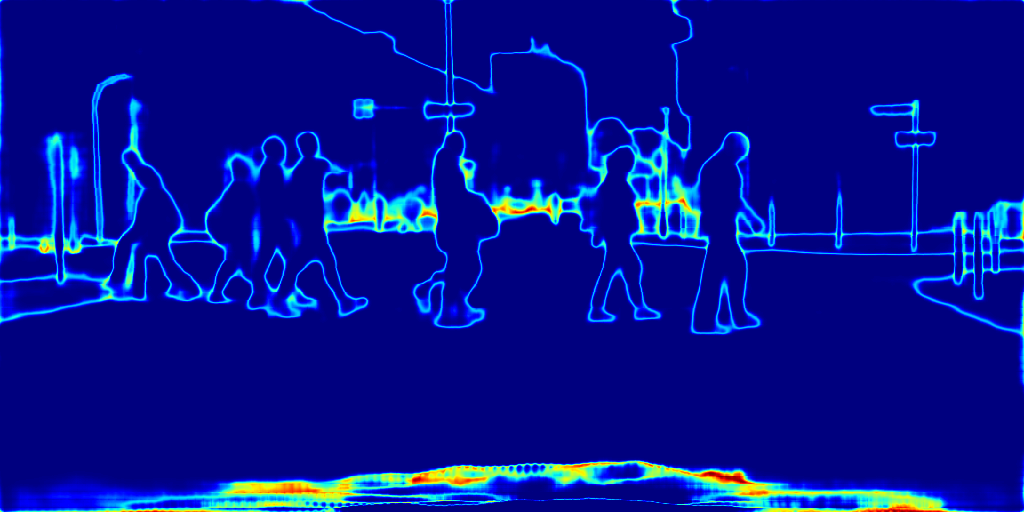
\includegraphics[width=0.32\textwidth,trim={0 20mm 0 0},clip]{Chapter2/Figs/results/segnet_107_output_2.png}
        \caption{Uncertainty --- understanding the prediction's confidence and what the model does not know. From left: input image, semantic segmentation, model uncertainty (where blue represents certain and more red colours are uncertain predictions). The model exhibits increased uncertainty in distance objects and around object boundaries.}
    \end{subfigure}
\caption[Examples of algorithms in this thesis.]{Examples of the variety of algorithms developed in this thesis. (a) shows a scene understanding system from \cref{scene_understanding}. (b) shows a localisation system which can determine the camera's 3D position and orientation in space from \cref{localisation}. (c) shows a semantic segmentation system which is aware of its uncertainty from \cref{scene_understanding}.}
\label{ch1:teaser}
\end{figure}

But end-to-end learning has problems too. It is often not good for data efficiency, interpretability or safety \citep{mcallister2017av_bdl}. This thesis makes two observations which challenge the weaknesses of end-to-end learning:
\begin{itemize}
\item We do not need to learn everything from scratch, we know many things about the world,
\item We cannot explain everything from our data and we need to know what our model does not know.
\end{itemize}
In this thesis, we focus on these ideas using concepts from \textbf{\textit{geometry}} and \textbf{\textit{uncertainty}}. These ideas are elaborated on in the next few sections.

\subsection{Machine Learning in Computer Vision}

Let us consider two arguments which motivate the use of machine learning approaches, in particular deep learning, to complicated computer vision problems.

First, as the most powerful demonstration of perception, how does the human visual pathway develop? Surprisingly, we are born without the ability to see \citep{gibson1960visual}. Infant humans learn through a mixture of semi-supervised and unsupervised learning \citep{kellman2006infant}. It typically takes three months to learn colour and depth perception. Object detection can take nine to twelve months. Suppose that an infant experiences one saccade (visual experience) per second of their first year of existence. This amounts to $1 \text{~saccade/s} \times 3600 \text{~sec/hour} \times 8 \text{~h/day} \times 365 \text{~days/year} = 10,000,000 \text{~training examples}$ in the first year of their life. Interestingly, this size is of the same order of magnitude as one of the largest computer vision datasets, ImageNet \citep{deng2009imagenet}. It is also the size of the data which is required for today’s image recognition models to achieve super-human performance \citep{he2016deep}. As our best example, the human visual system learns to see --- through nurture, not nature.

Secondly, it simply is not scalable to hand-design an algorithm
to support and adapt to complicated and dynamic data such as our visual world. Modern computer vision algorithms contain over 100 million parameters. Input data is very high dimensional, typically containing several million pixels being streamed over time. To date, we have been unable to specify hand-engineered rules to design top-performing architectures. To understand large amounts of data at scale we need to learn.

While there are many examples of machine learning models, \textit{deep convolutional neural networks} \citep{Fukushima1979neocognitron,krizhevsky2012imagenet} are most effective for vision tasks. Convolutional neural networks are a subset of deep learning which are particularly useful for computer vision because they are spatially invariant. Algorithms like stochastic gradient descent and backpropagation \citep{lecun88} can train networks containing millions of parameters. These networks can be optimised from a loss function formulated from supervised labelled training data or unsupervised learning.

Deep learning models have typically been restricted to classification settings. They excel at sub-sampling data and expanding feature dimensions to make classifications at an image level \citep{krizhevsky2012imagenet}. Applying these models to other problems in computer vision is more challenging. This is because other computer vision tasks require representations for recognition, registration or reconstruction \citep{cipolla2010computer}. Standard recognition encoder networks \citep{krizhevsky2012imagenet,simonyan2013deep,he2004multiscale} cannot be naively applied to these domains. This thesis proposes a broader range of deep learning architectures for many other computer vision problems.

Finally, there is an interesting comparison between deep learning models and the human visual system. The human visual cortex processes images from the retina initially through the V1-V4 and IT cortex \citep{hubel1962receptive}. Evidence shows that hierarchical representations are formed at increasing levels of abstraction (edges, lines, contours, objects, scenes) \citep{hubel1962receptive}. Similar levels of abstraction are seen with increasing convolutional neural network depth \citep{zeiler2014visualizing}.

\subsection{Geometry in Computer Vision}

Geometry is concerned with questions of shape, size, relative position of figures and the properties of space.
In computer vision, geometry is used to describe the structure and shape of the world. Specifically, it concerns measures such as depth, volume, shape, pose, disparity, motion or optical flow. We understand the mathematics of geometry very well \citep{koenderink1991solid,faugeras1993three,hartley2000}.
Consequently, there are a lot of complex relationships, such as depth and motion, which do not need to be learned from scratch with deep learning.
By building architectures which use this knowledge, we can simplify the learning problem.

The alternative paradigm to geometry is using semantic representations. 
Semantic representations use a language to describe relationships in the world. For example, we might describe an object as a `cat' or a `dog'.
Geometry has two attractive characteristics over semantics:
\begin{itemize}
\item Geometry can be directly observed. We see the world's geometry directly using vision.  At the most basic level, we can observe motion and depth directly from a video by following corresponding pixels between frames \citep{koenderink1991affine}.  Other interesting examples include observing shape from shading \citep{horn1989shape} or depth from stereo disparity \citep{scharstein2002taxonomy}. In contrast, semantic representations are often proprietary to a human language, with labels corresponding to a limited set of nouns, which cannot be directly observed from the world.
\item Geometry is based on continuous quantities. For example, we can measure depth in metres or disparity in pixels. In contrast, semantic representations are largely discretised quantities or binary labels.
\end{itemize}
With these properties, we show that we can use geometry to improve performance (\cref{localisation} and \cref{stereo}) and for unsupervised learning, without human-annotated labels (\cref{stereo} and \cref{motion}).

However, geometry alone cannot form a robust vision system. This is because models must learn representations which are robust to noise and outliers. Deep learning is powerful at learning representations which are robust to outliers and other nuisance variables. Additionally, models also need to be aware of the inherent uncertainty in the data.

\subsection{Uncertainty in Computer Vision}

Understanding what a model does not know is a critical part of many machine learning systems \citep{ghahramani2015probabilistic}. Uncertainty is important to improve trustworthiness and safety of these systems \citep{mcallister2017av_bdl}. Unfortunately, today's deep learning algorithms are usually unable to understand their uncertainty. These models are often taken blindly and assumed to be accurate, which is not always the case. For example, in two recent situations this has had disastrous consequences.

\begin{itemize}
\item In May 2016 the world tragically experienced the first fatality from an assisted driving system. According to the manufacturer's blog, `Neither Autopilot nor the driver noticed the white side of the tractor trailer against a brightly lit sky, so the brake was not applied' \citep{teslaCrashReport}.
\item In July 2015, an image classification system erroneously identified two African American humans as gorillas, raising concerns of racism and discrimination \citep{googleblackgorilla}.
\end{itemize}

If both these algorithms could assign a high level of uncertainty to their erroneous predictions, then each system may have been able to make better decisions and likely avoid disaster. Unfortunately, traditional machine learning approaches to understanding uncertainty, such as Gaussian processes \citep{rasmussen2006gaussian}, do not scale to high dimensional inputs like images and videos. 
To effectively understand this data, we need deep learning. But deep learning struggles to model uncertainty.

One of the techniques used in this thesis to model uncertainty is Bayesian deep learning \citep{mackay1992practical} which provides a deep learning framework which can model uncertainty.
Bayesian deep learning is a field at the intersection between deep learning and Bayesian probability theory.
It offers principled uncertainty estimates from deep learning architectures.
These deep architectures can model complex tasks by leveraging the hierarchical representation power of deep learning, while also being able to infer complex multi-modal posterior distributions.
Probabilistic deep learning models typically form uncertainty estimates by either placing distributions over model weights, or by learning a direct mapping to probabilistic outputs. In this thesis we show how to formulate accurate and scalable computer vision models which can understand the model's uncertainty with Bayesian deep learning.

\section{Contributions}

To summarise, the contributions of this thesis are as follows:
\begin{itemize}
\item We demonstrate how to formulate many challenging computer vision problems with end-to-end deep learning. We show the performance of these models significantly improves over traditional approaches.
\item We show how to improve performance of these models by leveraging the problem's geometry. We demonstrate that this reduces the amount of training data required and improves the generalisation of these models to novel examples.
\item Finally, for practical and safe systems, it is important to understand our model’s uncertainty. We show how to quantify uncertainty in deep learning computer vision models with Bayesian deep learning and probabilistic modelling.
\end{itemize}

\section{Co-Authored Papers}

Some extracts from this thesis appear in the following co-authored publications and preprints.
\cref{scene_understanding} contains work from:
\begin{itemize}
\item Vijay Badrinarayanan, Alex Kendall and Roberto Cipolla. SegNet: A Deep Convolutional Encoder-Decoder Architecture for Image Segmentation. IEEE Transactions on Pattern Analysis and Machine Intelligence, 2017.
\item Alex Kendall and Yarin Gal. What Uncertainties Do We Need in Bayesian Deep Learning for Computer Vision? Advances in Neural Information Processing Systems, 2017.
\item Alex Kendall, Yarin Gal and Roberto Cipolla. Multi-Task Learning Using Uncertainty to Weigh Losses for Scene Geometry and Semantics. arXiv preprint arXiv:1705.07115, 2017.
\end{itemize}
\cref{localisation} is adapted from:
\begin{itemize}
\item Alex Kendall, Matthew Grimes and Roberto Cipolla. PoseNet: A Convolutional Network for Real-Time 6-DOF Camera Relocalization. Proceedings of the International Conference on Computer Vision, 2015.
\item Alex Kendall and Roberto Cipolla. Modelling Uncertainty in Deep Learning for Camera Relocalization. Proceedings of the International Conference on Robotics and Automation, 2016.
\item Alex Kendall and Roberto Cipolla. Geometric loss functions for camera pose regression with deep learning. Proceedings of the IEEE Conference on Computer Vision and Pattern Recognition, 2017.
\end{itemize}
\cref{stereo} extends:
\begin{itemize}
\item Alex Kendall, Hayk Martirosyan, Saumitro Dasgupta, Peter Henry, Ryan Kennedy, Abraham Bachrach, and Adam Bry. End-to-End Learning of Geometry and Context for Deep Stereo Regression. Proceedings of the International Conference on Computer Vision, 2017.
\item Alex Kendall and Roberto Cipolla. Uncertainty and Unsupervised Learning for Stereo Vision. Under Review, 2017.
\end{itemize}
And finally, \cref{motion} is adapted from:
\begin{itemize}
\item Alex Kendall and Roberto Cipolla. VideoSegNet: Learning Motion and Geometry for Video Semantic Segmentation. Under Review, 2017.
\end{itemize}

\section{Thesis Structure}

The outline of the thesis is as follows. The following four chapters discuss core computer vision tasks: scene understanding in \cref{scene_understanding}, localisation in \cref{localisation}, stereo vision in \cref{stereo}, video and motion in \cref{motion}. For each chapter’s topic, we review the prior art. We introduce formulations for end-to-end deep learning architectures. We discuss how to improve these end-to-end models with notions of the problem’s geometry. Finally, we show how to capture model uncertainty. In \cref{conclusions}, we make overall conclusions, discuss the application of this technology and suggest directions for future research.